% =====================================================================================================
\section{Hardware Architecture}\label{sec:hardware}
\begin{figure*}[t]
\centering
\resizebox{\textwidth}{!}{% Fabric datapath of the contract-v3 lane encoder (rtl/secure_jpeg_lanes_top.v, rtl/encoder_lane.v).
% Bus widths are the RTL port widths; module names are the RTL file names.
\begin{tikzpicture}[x=1cm, y=1cm, st/.style={pl, minimum height=9mm, minimum width=13.5mm, font=\tiny}]
% ---- input and dealer
\node[blk, fill=netfill, font=\tiny, minimum height=9mm] (in) at (0,0) {s\_axis\\64\,b\\2 px/beat};
\node[pl, font=\tiny, minimum height=24mm, minimum width=11mm, align=center] (deal) at (1.45,-0.75) {dealer\\[2pt]MCU row\\$r\to$ lane\\$r \bmod L$};
\draw[bus] (in) -- (in -| deal.west);
% ---- lane 0 (full) -- y = 0
\node[st] (cc0)  at (3.05,0) {rgb2ycbcr\\2px $\to$ 1\\sample/clk};
\node[st] (dct0) at (4.65,0) {dct8x8\\two-pass\\13-bit};
\node[st] (q0)   at (6.25,0) {quantiser\\$\times R_{uv}$,\\$\gg 16$};
\node[st] (zz0)  at (7.85,0) {zigzag\_rle\\DC pred.\\reset/seg.};
\node[st, fill=cryfill] (se0) at (9.45,0) {selective\\\_enc\\(XOR)};
\node[st] (hu0)  at (11.05,0) {huffman\\\_enc\\(Annex K)};
\node[st] (bp0)  at (12.65,0) {bit\_packer\\stuff, pad\\per seg.};
\node[st, minimum width=10mm] (ff0)  at (14.05,0) {byte\\FIFO\\2\,KB};
\node[cry, font=\tiny, minimum width=19mm, minimum height=8mm] (ks0) at (9.45,1.25) {keystream\_gen\\Ascon$(K_{\mathrm{seg}}, N_{s,t})$};
\draw[arr] (ks0) -- node[lbl, left, align=right]{16-bit window,\\take $n\le 12$ bits} (se0);
\draw[arr] (deal.east |- cc0) -- (cc0);
\draw[arr] (cc0) -- node[lbl, above]{8} (dct0);
\draw[arr] (dct0) -- node[lbl, above]{16} (q0);
\draw[arr] (q0) -- node[lbl, above]{16} (zz0);
\draw[arr] (zz0) -- node[lbl, above]{20} (se0);
\draw[arr] (se0) -- node[lbl, above]{20} (hu0);
\draw[arr] (hu0) -- node[lbl, above]{32} (bp0);
\draw[arr] (bp0) -- node[lbl, above]{8} (ff0);
\begin{scope}[on background layer]
\node[grp, fill=plfill!30, fit=(cc0)(ff0)(ks0), inner sep=1.6mm, label={[font=\tiny\bfseries, anchor=south west, inner sep=1pt]north west:encoder\_lane 0}] (lane0) {};
\end{scope}
% ---- lane L-1 (collapsed) -- y = -1.6
\node[pl, font=\tiny, text width=118mm, minimum height=7mm, align=center] (laneL) at (8.46,-1.8) {the same pipeline (colour, DCT, quantiser, zig-zag + RLE, \textbf{selective XOR}, Huffman, packer, FIFO) with its own keystream generator};
\node[font=\tiny\bfseries, anchor=south west] at (laneL.north west) {encoder\_lane $L{-}1$ \ (lanes $1 \ldots L{-}1$; $L = 1, 2, 4$)};
\draw[arr] (deal.east |- laneL) -- (laneL);
% ---- merger, tag, word packer
\node[pl, font=\tiny, minimum height=24mm, minimum width=13mm, align=center] (mrg) at (16.0,-0.75) {segment\\\_merger\\[2pt]seg.\ $s$ from\\lane $s \bmod L$\\(E5: $\lfloor s/c\rfloor$\\$\bmod L$)\\[2pt]+ RST$_{s \bmod 8}$};
\draw[arr] (ff0.east) -- (ff0.east -| mrg.west);
\draw[arr] (laneL.east) -- (laneL.east -| mrg.west);
\node[cry, font=\tiny, minimum width=18mm, minimum height=9mm] (tag) at (18.15,0.35) {tag\_unit\\Ascon MAC over\\prefix $\|$ scan};
\node[pl, font=\tiny, minimum width=18mm, minimum height=9mm] (wp) at (18.15,-1.85) {scan\_word\\\_packer\\32\,b + TKEEP};
\draw[arr] (mrg.east |- tag) -- node[lbl, above]{8} (tag.west);
\draw[arr] (mrg.east |- wp) -- node[lbl, above]{8} (wp.west);
\node[blk, fill=netfill, font=\tiny, minimum height=8mm] (out) at (18.15,-3.1) {m\_axis 32\,b};
\draw[bus] (wp) -- (out);
% ---- per-frame key, registers
\node[cry, font=\tiny, minimum width=24mm, minimum height=8mm] (kseg) at (5.6,2.85) {kseg\_unit: $K_{\mathrm{seg}}$ =\\Ascon-MAC$(K, N^{\mathrm{enc}}_t, \text{``lanes''})$};
\draw[arr] (kseg.east) -| node[lbl, pos=0.75, right]{$K_{\mathrm{seg}}$, once per frame, to every lane} (ks0.north);
\node[pl, font=\tiny, minimum width=24mm, minimum height=8mm] (regs) at (1.6,2.85) {axil\_regs\\$K$, $\sigma$, $t$, mode, size, $R_{uv}$};
\draw[arr] (regs) -- (kseg);
\draw[arr] (regs.north) -- ++(0,0.3) -| node[lbl, pos=0.25, above]{$K$ and the 26-byte prefix (mode, $\sigma$, $t$, $W$, $H$)} (tag.north);
\draw[arr] (tag.south) ++(0.5,0) -- ++(0,-0.35) node[lbl, right]{$T$ to TAG0--3};
\end{tikzpicture}
}
\caption{Fabric datapath of the lane encoder \texttt{secure\_jpeg\_lanes\_top} (module names are the RTL files; numbers on arrows are bus widths in bits). The dealer sends MCU row $r$ to lane $r \bmod L$; each lane converts two pixels per clock into one sample per clock, transforms, quantizes and entropy-codes its restart segments with its own keystream; the merger restores raster order and inserts restart markers; the tag unit authenticates the 26-byte prefix and the merged scan; the word packer writes 32-bit words to the DMA. The single-pipeline encoder \texttt{secure\_jpeg\_top} is one lane without dealer and merger, with one keystream per frame.}
\label{fig:pl}
\end{figure*}

\subsection{Datapath}\label{sec:datapath}
Fig.~\ref{fig:pl} shows the encoder. All stages are joined by valid/ready handshakes: data moves on a rising edge where both are high, a sender holds its data while valid is high and ready is low, and valid never depends on ready. Every stage therefore tolerates back-pressure from the DMA without losing or corrupting data, which the testbenches check with random stalls on every interface.

\textit{Colour conversion and line buffers.} \texttt{rgb2ycbcr\_2px} takes two pixels per clock from the 64-bit stream, applies~\eqref{eq:ycc} with three multiply-add trees per pixel (the luma line buffer is split into even and odd banks so that both pixels are written in one clock), averages chroma and writes an MCU row (16 lines) into block-RAM line buffers sized for 2048-pixel lines (1024 with four lanes). It reads the samples back block by block in the order Y0 Y1 Y2 Y3 Cb Cr, one sample per clock. Its buffers hold all block RAM of the encoder.

\textit{Transform and quantizer.} \texttt{dct8x8} computes~\eqref{eq:dct} as two passes of an eight-tap multiply-accumulate with a transpose buffer between them, one sample per clock; the row sums are pipelined over five stages. \texttt{quantiser} implements~\eqref{eq:quant} with one DSP multiplication by the reciprocal table, which the ARM writes through the register map once per session.

\textit{Zig-zag, run-length and DC coding.} \texttt{zigzag\_rle} stores the coefficients of a block in zig-zag order, takes the DC difference with one predictor per component, and emits symbols (is\_dc, run, $s$, $\amp$, EOB, component, frame-last), at most one per clock. Its predictors reset at every restart segment.

\textit{Encryption.} \texttt{selective\_enc} implements~\eqref{eq:selenc} (Section~\ref{sec:circuit}). \texttt{huffman\_enc} maps each symbol to a right-aligned chunk of up to 27 bits (code followed by the field) from the Annex~K tables, and \texttt{bit\_packer} assembles bytes, inserts the 0x00 after every 0xFF, and at the end of a segment pads with 1-bits and marks the last byte.

\textit{Merger, tag and output.} \texttt{segment\_merger} copies segment $s$ byte by byte from its lane's FIFO until the byte marked last, then writes 0xFF, 0xD0 $+ (s \bmod 8)$ unless $s$ is the last segment, and moves to the next lane. \texttt{tag\_unit} absorbs the prefix and every merged byte into an Ascon core; \texttt{scan\_word\_packer} packs bytes into 32-bit little-endian words with TKEEP and TLAST and counts them for the OUT\_BYTES register.

\subsection{Circuit of the encryption stage}\label{sec:circuit}
\begin{figure}[t]
\centering
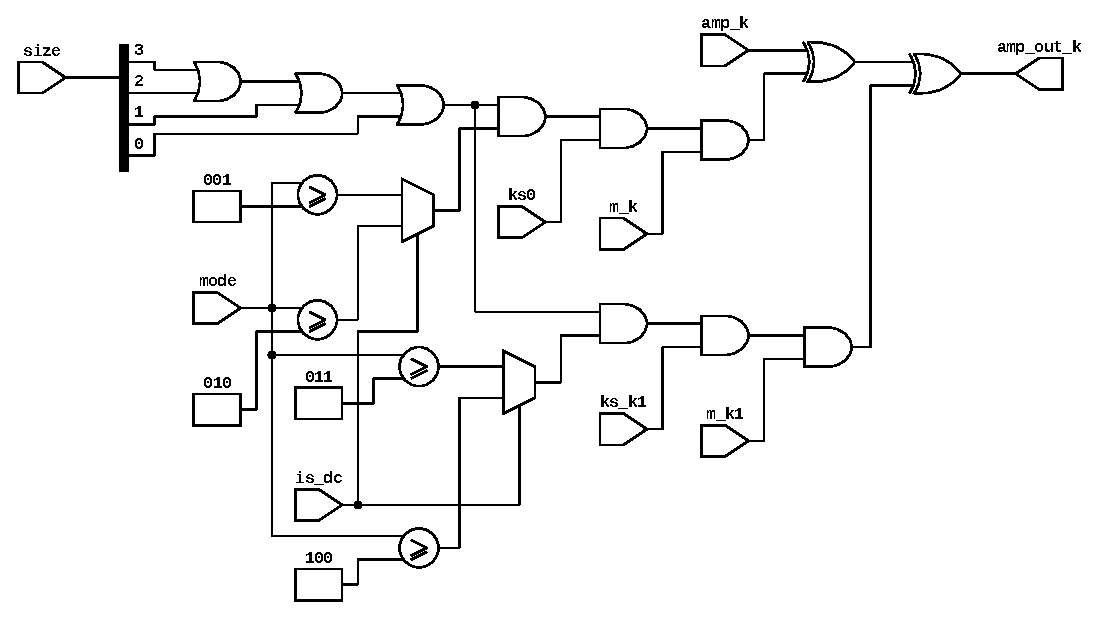
\includegraphics[width=\columnwidth]{figures/fig_selective_enc_bitslice.pdf}
\caption{Gate-level circuit of bit slice $k$ of \texttt{selective\_enc.v}, generated from the RTL by Yosys and netlistsvg. The OR of the size bits gives $[s \ne 0]$; comparators on the mode and two multiplexers selected by is\_dc form the sign enable $\gamma$ (upper path) and the amplitude enable $\alpha$ (lower path); the two XORs implement~\eqref{eq:slice}. $m_k = [k < s]$ and $m_{k+1}$ are bits of the mask $2^s - 1$; ks0 and ks\_k1 are bits 0 and $k{+}1$ of the keystream window. A test simulates the slice exhaustively and compares it with the golden model.}
\label{fig:circuit}
\end{figure}
Fig.~\ref{fig:circuit} is one bit slice of the stage at gate level, generated from its RTL; the handshake around it is described by the equations below. The control part decodes $\gamma = [s \ne 0] \wedge (\text{is\_dc} \mathbin{?} \text{mode} \ge 2 : \text{mode} \ge 1)$ and $\alpha = [s \ne 0] \wedge (\text{is\_dc} \mathbin{?} \text{mode} \ge 4 : \text{mode} \ge 3)$; mode 5 selects the same fields as mode 4 because all comparisons are $\ge$. The data part is eleven identical bit slices,
\begin{equation}
\amp'_k = \amp_k \xor (\gamma z_0 \wedge m_k) \xor (\alpha z_{k+1} \wedge m_{k+1}), \quad m = 2^s - 1,
\label{eq:slice}
\end{equation}
one XOR gate deep after the masks, so the stage closes timing with room to spare. The handshake accepts a symbol when $i_{\mathrm{ready}} = (\neg o_{\mathrm{valid}} \vee o_{\mathrm{ready}}) \wedge (k_{\mathrm{avail}} \ge n)$ and signals the keystream generator to advance by $n$ bits.

\textit{Keystream window.} \texttt{keystream\_gen} holds two 128-bit slots, the block being consumed ($u$) and the next one ($u'$), and a pointer $p \in [0, 127]$ to the next unused bit. It presents the 16-bit window $(u' \cat u) \gg p$ and its fill level $k_{\mathrm{avail}} = \min(16, 128 - p + 128\,[u' \text{ valid}])$; taking $n$ bits sets $p \leftarrow p + n$, and when $p$ passes 128 the next slot moves in. A new block is requested whenever fewer than two are held or in flight, so the core runs ahead of the consumer.

\begin{proposition}[The cipher never stalls the encoder]\label{prop:supply}
Once the first keystream block of a segment is available, the encryption stage never waits for keystream bits.
\end{proposition}
\begin{IEEEproof}
The stage accepts at most one symbol per clock and takes $n \le 11$ bits per symbol~\eqref{eq:need}, so the demand never exceeds 11 bits per cycle. The core produces 128 bits per data block in nine cycles (one cycle to absorb, eight rounds of $p^8$), i.e.\ $128/9 > 14$ bits per cycle, and it keeps up to 256 bits buffered, more than the 16 that the window exposes. Supply exceeds the worst-case demand, so the window, once filled, can never drop below the 11 bits a symbol needs.
\end{IEEEproof}
The first block costs an initialization ($p^{12}$, 12 cycles) and one data block (nine cycles). At the start of a frame this overlaps with filling the first MCU row (16 lines), so it is invisible; RTL simulation confirms that the cycle counts of E0--E4 differ by at most \MaxExtraCycles{} cycles per frame. In the lane encoder every segment restarts its keystream, and in E5 every MCU does; a segment of one MCU takes at least 384 cycles, so a 21-cycle restart overlapped with the previous segment costs a few per cent of throughput, which we measure in Section~\ref{sec:hwresults}.

\subsection{Ascon core}\label{sec:asconcore}
\begin{figure}[t]
\centering
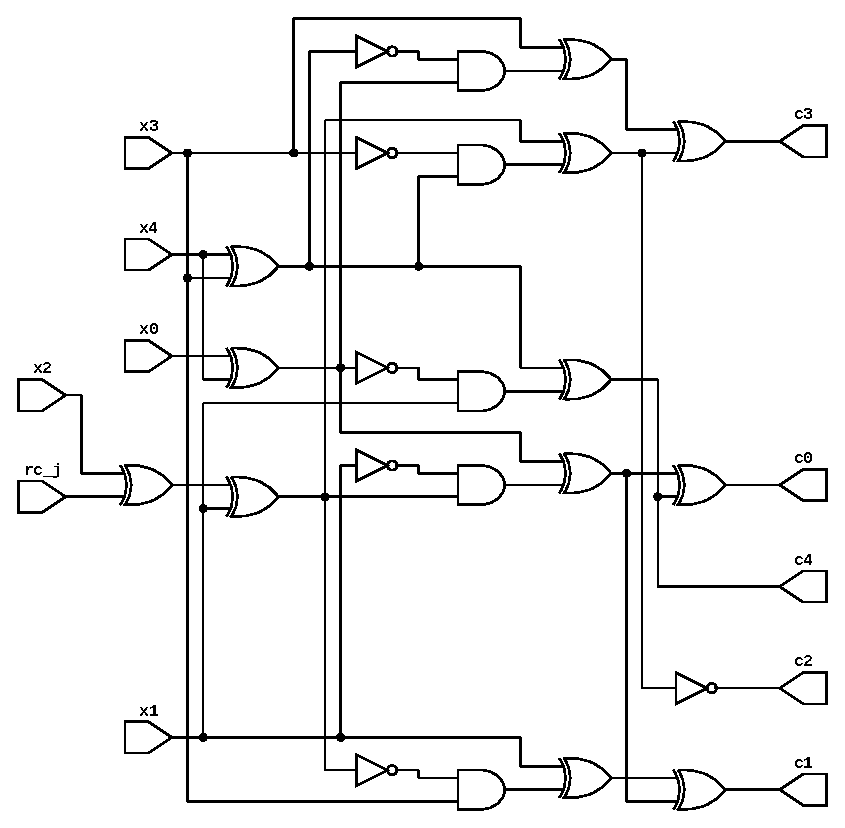
\includegraphics[width=\columnwidth]{figures/fig_ascon_sbox_slice.pdf}
\caption{One of the 64 bit slices of the Ascon round of \texttt{ascon\_round.v} ($p_C$ and $p_S$), generated from the RTL by Yosys and netlistsvg: twelve XOR (one for the round-constant bit rc\_j, zero for $j \ge 8$), five AND and six NOT gates. The linear layer $p_L$ acts on whole 64-bit words (two rotations and two XORs per bit). A test checks that 64 such slices followed by $p_L$ reproduce a round of the golden model.}
\label{fig:asconslice}
\end{figure}
\texttt{ascon\_aead128\_core} computes one round per clock cycle: a 320-bit state register, a 4-bit round counter $r$ and the combinational round of Fig.~\ref{fig:asconslice}, with the round constant $c = \bar r \cat r$ (eight bits, $\bar r$ the complement of $r$), which equals $16(15 - i) + i$ for round $i$. The $p^{12}$ permutation counts $r$ from 0 to 11, the $p^8$ permutation from 4 to 11. Counting the operators of \texttt{ascon\_round.v}, one bit slice of $p_S$ has 22 gates (eleven XOR, five AND, six NOT), so $p_S$ is $64 \times 22 = 1408$ gates, $p_L$ adds $2 \times 320$ two-input XORs and $p_C$ eight. A block interface accepts associated data and message blocks with byte masks and the padding rule of the standard; the same core serves as keystream generator (message blocks of zeros, never finalized), as MAC (associated data only, empty message) and as key-derivation unit. The design instantiates one core per lane for keystreams, one for the segment key and one for the tag.

\textit{Tag unit.} \texttt{tag\_unit} latches the 26-byte prefix at frame start, absorbs it, then gathers scan bytes into 128-bit blocks. A block of 16 bytes arrives in at least 16 cycles at one byte per clock, while absorbing it takes nine, so the tag unit never slows the merger; the final partial block, the empty message and the $p^{12}$ finalization add a fixed number of cycles after the last byte.

\subsection{Parallel lanes}\label{sec:lanes}
One pipeline consumes one sample per clock; with 1.5 samples per pixel it needs at least 1.5 cycles per pixel. Restart segments are independent (DC predictors reset, byte alignment, own keystream~\eqref{eq:zs}), so $L$ copies of the pipeline can code segments simultaneously: the dealer sends MCU row $r$ to lane $r \bmod L$ and the merger reads segment $s$ from lane $s \bmod L$ (in E5, segment $s$ belongs to MCU row $\lfloor s/c \rfloor$ with $c = W/16$ MCUs per row, so it comes from lane $\lfloor s/c \rfloor \bmod L$, tracked with row and column counters instead of a divider). The 64-bit input bus brings two pixels per clock. The cost per pixel is therefore bounded below by
\begin{equation}
c_L \ge \max\Bigl(\frac{1.5}{L}, \frac{1}{2}\Bigr), \qquad \Theta_L = \frac{f_{\mathrm{clk}}}{c_L},
\label{eq:lanes}
\end{equation}
i.e.\ \BoundOneCpp, \BoundTwoCpp{} and \BoundFourCpp{} cycles per pixel, or at most \BoundOneMpix, \BoundTwoMpix{} and \BoundFourMpix\,Mpixel/s at 100\,MHz for $L = 1, 2, 4$; beyond four lanes the input bus, not the encoder, is the limit. Two costs come on top. Before the first MCU row is complete no block can be transformed, which for a single pipeline gives the measured law
\begin{equation}
c_1(r) = 1.5 + \frac{A}{r}, \qquad A = \FillA,
\label{eq:fill}
\end{equation}
for a frame of $r$ MCU rows; and each segment adds a keystream restart and a byte flush. The bytes do not depend on $L$, because segments are merged in raster order and each one depends only on its own pixels and keystream.

\subsection{Register map and driver}\label{sec:regs}
\begin{table}[t]
\caption{AXI4-Lite register map (32-bit; \texttt{axil\_regs.v}).}
\label{tab:regs}
\centering\small\setlength{\tabcolsep}{3pt}
\begin{tabular}{lll}
\toprule
Offset & Name & Function \\
\midrule
0x00 & CTRL & bit 0 START (self-clearing), bits 3:1 level E0--E5 \\
0x04 & STATUS & DONE, BUSY, TAG\_VALID \\
0x08 & VERSION & 0x5EC0\_0200 (single pipeline); 0x5EC0\_03LL ($L$ lanes, bit 7 = E5) \\
0x10, 0x14 & WIDTH, HEIGHT & pixels (multiples of 16) \\
0x18, 0x50 & FRAME\_CTR (lo, hi) & 63-bit frame counter $t$ \\
0x1C, 0x4C & SESSION\_ID (lo, hi) & 64-bit session identifier $\sigma$ \\
0x20--0x2C & KEY0--3 & video key $K_e$ (write-only) \\
0x30 & OUT\_BYTES & scan bytes of the last frame \\
0x34--0x40 & TAG0--3 & tag $T_t$ \\
0x44, 0x48 & QT\_ADDR, QT\_DATA & 17-bit reciprocals $R(u, v)$ \\
\bottomrule
\end{tabular}
\end{table}
Table~\ref{tab:regs} gives the register map. Once per session the driver writes the key, the session identifier and the 128 reciprocals; per frame it writes the size and the counter, sets CTRL to $1 + 2 \cdot \text{level}$, starts the DMA receive and send channels, waits for DONE, and reads OUT\_BYTES and the tag. The VERSION register tells the driver which contract the bitstream implements: bit 7 says that the fabric codes E5 segments, and only then does the driver allow level E5.

\subsection{PYNQ-Z2 system}\label{sec:zynq}
\begin{figure*}[t]
\centering
\resizebox{\textwidth}{!}{% PYNQ-Z2 block design as built by future_work/board/block_design.tcl (cell names as in the Vivado
% utilisation report: ps7, ps7_axi_periph, axi_mem_intercon, dma, sjpeg, irq_concat, proc_sys_reset).
% Clock, reset and interrupt nets are drawn as net labels, as Vivado's diagram does.
\begin{tikzpicture}[x=1cm, y=1cm,
  cell/.style={draw=inkc, fill=white, rounded corners=1pt, align=center, font=\tiny, inner sep=2pt},
  port/.style={font=\tiny, inner sep=1pt},
  net/.style={font=\tiny\itshape, inner sep=1pt, text=inkc!75},
  axi/.style={-{Latex[length=1.4mm]}, line width=1.0pt, inkc},
  axis/.style={-{Latex[length=1.4mm]}, line width=1.0pt, inkc, densely dashed},
  sg/.style={inkc!75, line width=0.4pt, -{Latex[length=1.1mm]}}]
% ---- PS7
\node[cell, fill=psfill, minimum width=32mm, minimum height=48mm] (ps) at (0,-0.15) {};
\node[font=\scriptsize\bfseries, anchor=north] at (ps.north) {ps7};
\node[font=\tiny, anchor=north, align=center] at ([yshift=-3.5mm]ps.north) {ZYNQ7 Processing System\\2$\times$ Cortex-A9, DDR ctrl.};
\coordinate (pGP) at (1.6,1.3);  \node[port, anchor=east] at (pGP) {M\_AXI\_GP0};
\coordinate (pHP) at (1.6,0.1);  \node[port, anchor=east] at (pHP) {S\_AXI\_HP0 (64\,b)};
\coordinate (pCK) at (1.6,-0.7); \node[port, anchor=east] at (pCK) {FCLK\_CLK0};
\coordinate (pRS) at (1.6,-1.15); \node[port, anchor=east] at (pRS) {FCLK\_RESET0\_N};
\coordinate (pIQ) at (1.6,-1.6); \node[port, anchor=east] at (pIQ) {IRQ\_F2P};
\coordinate (pDD) at (-1.6,0.6); \node[port, anchor=west] at (pDD) {DDR};
\coordinate (pFI) at (-1.6,0.1); \node[port, anchor=west] at (pFI) {FIXED\_IO};
\draw[sg] (pDD) -- ++(-0.5,0) node[port, left]{DDR3, 512\,MB};
\draw[sg] (pFI) -- ++(-0.5,0) node[port, left, align=right]{MIO: UART,\\Ethernet, SD card};
\draw[sg] (pCK) -- ++(0.5,0) node[net, right]{clk (100\,MHz) $\to$ every cell};
% ---- interconnects
\node[cell, minimum width=24mm, minimum height=9mm] (per) at (4.7,1.3) {\textbf{ps7\_axi\_periph}\\AXI interconnect\\S00 $\to$ M00, M01};
\node[cell, minimum width=24mm, minimum height=9mm] (mem) at (4.7,0.1) {\textbf{axi\_mem\_intercon}\\AXI interconnect\\S00, S01 $\to$ M00};
\draw[axi] (pGP) -- (per.west);
\draw[axi] (mem.west) -- (pHP);
% ---- DMA
\node[cell, fill=plfill, minimum width=34mm, minimum height=31mm] (dma) at (8.8,0.4) {};
\node[font=\scriptsize\bfseries, anchor=north] at (dma.north) {dma};
\node[font=\tiny, anchor=north] at ([yshift=-3.3mm]dma.north) {AXI DMA (simple mode)};
\coordinate (dL) at (7.1,1.0);   \node[port, anchor=west] at (dL) {S\_AXI\_LITE};
\coordinate (dM) at (7.1,-0.35);   \node[port, anchor=west] at (dM) {M\_AXI\_MM2S};
\coordinate (dS) at (7.1,-0.75);  \node[port, anchor=west] at (dS) {M\_AXI\_S2MM};
\coordinate (dA) at (10.5,0.75);  \node[port, anchor=east] at (dA) {M\_AXIS\_MM2S (64\,b)};
\coordinate (dB) at (10.5,0.3);  \node[port, anchor=east] at (dB) {S\_AXIS\_S2MM (32\,b)};
\coordinate (dI1) at (10.5,-0.4); \node[port, anchor=east] at (dI1) {mm2s\_introut};
\coordinate (dI2) at (10.5,-0.75); \node[port, anchor=east] at (dI2) {s2mm\_introut};
\draw[axi] (per.east) -- ++(0.35,0) |- (dL);
\draw[axi] (dM) -- ++(-0.45,0) |- ([yshift=1.2mm]mem.east);
\draw[axi] (dS) -- ++(-0.3,0) |- ([yshift=-1.2mm]mem.east);
\draw[sg] (dI1) -- ++(0.35,0) node[net, right]{irq1};
\draw[sg] (dI2) -- ++(0.35,0) node[net, right]{irq2};
% ---- our IP
\node[cell, fill=cryfill!70, minimum width=33mm, minimum height=31mm] (sj) at (14.05,0.4) {};
\node[font=\scriptsize\bfseries, anchor=north] at (sj.north) {sjpeg};
\node[font=\tiny, anchor=north, align=center] at ([yshift=-3.3mm]sj.north) {secure\_jpeg\_lanes\_top\\(our RTL, module reference)};
\coordinate (sL) at (12.4,1.0); \node[port, anchor=west] at (sL) {s\_axil};
\coordinate (sA) at (12.4,0.75);  \node[port, anchor=west] at (sA) {s\_axis};
\coordinate (sB) at (12.4,0.3);  \node[port, anchor=west] at (sB) {m\_axis};
\coordinate (sK) at (15.7,0.75);  \node[port, anchor=east] at (sK) {clk};
\coordinate (sR) at (15.7,0.35);  \node[port, anchor=east] at (sR) {rst};
\coordinate (sI) at (15.7,-0.05);  \node[port, anchor=east] at (sI) {irq\_done};
\draw[axis] (dA) -- (sA);
\draw[axis] (sB) -- (dB);
\draw[axi] ([yshift=2mm]per.east) -- ++(0.6,0) |- (11.9,2.35) |- (sL);
\node[net, anchor=south] at (9.5,2.35) {M01: register map (Table~\ref{tab:regs})};
\draw[sg] (sK) ++(0.45,0) node[net, right]{clk} -- (sK);
\draw[sg] (sR) ++(0.45,0) node[net, right]{rst} -- (sR);
\draw[sg] (sI) -- ++(0.35,0) node[net, right]{irq0};
% ---- reset and interrupt helpers
\node[cell, minimum width=24mm, minimum height=7mm] (rst) at (4.7,-1.15) {\textbf{proc\_sys\_reset}};
\draw[sg] (pRS) -- (rst.west);
\draw[sg] (rst.east) -- ++(0.35,0) node[net, right]{rst};
\node[cell, minimum width=24mm, minimum height=7mm] (cc) at (4.7,-2.05) {\textbf{irq\_concat} (xlconcat)};
\draw[sg] (cc.west) -- ++(-0.6,0) |- (pIQ);
\node[net, anchor=west] (cin) at ([xshift=1.5mm]cc.east) {$\leftarrow$ \{irq2, irq1, irq0\}};
% ---- legend
\draw[axi] (7.3,-2.6) -- ++(0.5,0) node[port, right]{AXI4 / AXI4-Lite};
\draw[axis] (9.9,-2.6) -- ++(0.5,0) node[port, right]{AXI4-Stream};
\draw[sg] (12.1,-2.6) -- ++(0.5,0) node[port, right]{clock, reset, IRQ (net labels)};
\end{tikzpicture}
}
\caption{Block design of the PYNQ-Z2 system as built by our script. The processing system clocks the fabric at 100\,MHz (FCLK\_CLK0), controls the DMA and the encoder over M\_AXI\_GP0 and an AXI interconnect, and gives the DMA access to DDR over the 64-bit high-performance port S\_AXI\_HP0. The DMA streams pixels into the encoder (64 bits, two pixels per beat) and scan words out of it (32 bits). Interrupts of the encoder and both DMA channels are concatenated into IRQ\_F2P; the reset block drives the encoder's active-high synchronous reset.}
\label{fig:zynq}
\end{figure*}
Fig.~\ref{fig:zynq} shows the system around the encoder. A script builds it in Vivado from the RTL (the encoder enters as a module reference, without packaging), runs synthesis, place and route and bitstream generation, and exports the hardware handoff file that the PYNQ framework reads to find the IP blocks by name. The DMA runs in simple (register) mode; the driver allocates physically contiguous buffers, copies a frame into the input buffer, and starts both channels. Everything in the system runs on one clock, which avoids clock-domain crossings.

\subsection{Timing closure}\label{sec:timing}
Three lessons from the Vivado runs are worth recording. The first implementation met timing in simulation but reached only about 47\,MHz after routing, because the DCT summed a full row in one clock; splitting the sums over five pipeline stages with a stall-able handshake restored 100\,MHz without changing an output bit. The second appeared only in the complete Zynq system: the DMA's output register fed the colour conversion, clamp and line-buffer write in one clock. Registering the pixel, the multiply-add sums and the clamped result moved the writes three clocks later in the same order. The third came with the lanes: the zig-zag stage, which formed the zig-zag address, read the block buffer, took the DC difference and derived the size category and field in one clock, had been the critical path of the single pipeline with tens of picoseconds of slack, and missed 100\,MHz in the two-lane system. Storing coefficients in zig-zag order and splitting the coding into two handshaked stages closed timing for every configuration and raised the encoder's slack to $+$\TopWns\,ns; at 125\,MHz the \TopLimitAtOneTwoFive{} is now the limit (WNS \TopWnsAtOneTwoFive\,ns). In all three cases the golden model was the referee: a fix was accepted only when every RTL test still matched it bit for bit.
